\documentclass[12pt,a4paper,oneside]{book}

% Packages
\usepackage[utf8]{inputenc}
\usepackage[left=0.75in,right=0.75in,top=0.75in,bottom=1in]{geometry}
\usepackage{xcolor}
\usepackage{tikz}
\usetikzlibrary{shapes.geometric,shadows,patterns,positioning}
\usepackage{enumitem}
\usepackage{tcolorbox}
\usepackage{helvet}
\usepackage{setspace}
\usepackage{fancyhdr}
\usepackage{graphicx}
\usepackage{listings}
\usepackage{lstautogobble}

% Font settings
\renewcommand{\familydefault}{\sfdefault}
\setstretch{1.15}

% Define colors
\definecolor{headerred}{RGB}{213,43,30}
\definecolor{jsyellow}{RGB}{247,223,30}
\definecolor{cssblue}{RGB}{38,77,228}
\definecolor{htmlorange}{RGB}{228,77,38}
\definecolor{codebg}{RGB}{245,245,245}
\definecolor{codecomment}{RGB}{0,128,0}
\definecolor{codekeyword}{RGB}{0,0,255}
\definecolor{codestring}{RGB}{163,21,21}

% Listings settings for advanced look
\lstset{
    backgroundcolor=\color{codebg},
    basicstyle=\ttfamily\small,
    breaklines=true,
    frame=single,
    frameround=tttt,
    framexleftmargin=5pt,
    numbers=left,
    numberstyle=\tiny\color{gray},
    numbersep=8pt,
    showstringspaces=false,
    keywordstyle=\color{codekeyword}\bfseries,
    commentstyle=\color{codecomment}\itshape,
    stringstyle=\color{codestring},
    tabsize=2,
    autogobble=true,
    captionpos=t,
    xleftmargin=15pt,
    framexleftmargin=10pt,
    framexrightmargin=5pt,
    framextopmargin=5pt,
    framexbottommargin=5pt,
    rulecolor=\color{gray!30},
    aboveskip=15pt,
    belowskip=10pt
}

% JavaScript style
\lstdefinestyle{javascript}{
    language=Java,
    morekeywords={let, const, async, await, of, function, var, return, if, else, for, while, do, switch, case, break, continue, new, this, typeof, instanceof, true, false, null, undefined, class, extends, import, export, default, from, as, static, get, set, constructor, super, yield, promise, resolve, reject, then, catch, finally},
    morecomment=[l]{//},
    morecomment=[s]{/*}{*/},
    morestring=[b]',
    morestring=[b]",
    morestring=[b]`,
    keywordstyle=\color{blue!70!black}\bfseries,
    commentstyle=\color{green!50!black}\itshape,
    stringstyle=\color{orange!80!black},
    backgroundcolor=\color{blue!3},
    frame=shadowbox,
    rulesepcolor=\color{blue!20!gray!20},
    escapeinside={(*@}{@*)}
}

% Custom chapter command
\newcommand{\mychapter}[1]{%
    \clearpage
    \stepcounter{chapter}
    \vspace*{-1in}
    \begin{tcolorbox}[
        colback=headerred,
        coltext=white,
        boxrule=0pt,
        arc=0pt,
        outer arc=0pt,
        left=0pt,
        right=0pt,
        top=30pt,
        bottom=30pt,
        width=\textwidth,
        enlarge left by=-0.75in,
        enlarge right by=-0.75in,
        width=\paperwidth
    ]
        \centering
        \Huge\bfseries \thechapter.~#1
    \end{tcolorbox}
    \vspace{1em}
    \addcontentsline{toc}{chapter}{\protect\numberline{\thechapter}#1}
}

% Section formatting
\newcommand{\mysection}[1]{%
    \vspace{0.3em}
    {\large\bfseries\underline{#1}}
    \vspace{0.2em}
    \addcontentsline{toc}{section}{#1}
}

% Subsection formatting
\newcommand{\mysubsection}[1]{%
    \vspace{0.2em}
    {\normalsize\bfseries #1}
    \vspace{0.1em}
    \addcontentsline{toc}{subsection}{#1}
}

% Subsubsection formatting
\newcommand{\mysubsubsection}[1]{%
    \vspace{0.1em}
    {\normalsize\itshape #1}
    \vspace{0.1em}
}

% Page styles
\pagestyle{fancy}
\fancyhf{}
\fancyhead[C]{Full Stack Development}
\fancyfoot[C]{\thepage}
\renewcommand{\headrulewidth}{0pt}
\renewcommand{\footrulewidth}{0pt}

\fancypagestyle{plain}{
    \fancyhf{}
    \fancyfoot[C]{\thepage}
}

% Custom itemize
\setlist[itemize]{
    topsep=0.2em,
    itemsep=0.2em,
    parsep=0pt,
    partopsep=0pt,
    leftmargin=2em,
    label=\textbullet
}

\begin{document}
\frontmatter

% Title Page
\thispagestyle{empty}
\begin{titlepage}
    \begin{tikzpicture}[remember picture,overlay]
        \fill[headerred!10] (current page.north west) rectangle (current page.south east);
        \draw[headerred!30, line width=1pt] 
            ([xshift=1cm,yshift=-1cm]current page.north west) 
            rectangle ([xshift=-1cm,yshift=1cm]current page.south east);
    \end{tikzpicture}
    
    \vspace*{1cm}
    
    \begin{center}
        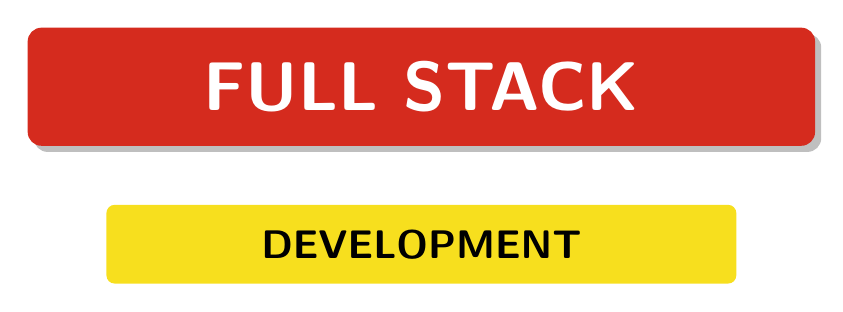
\begin{tikzpicture}
            \node[draw=none, fill=headerred, minimum width=10cm, minimum height=1.5cm, 
                  rounded corners=5pt, drop shadow] at (0,0) {
                \color{white}\Huge\bfseries FULL STACK
            };
            \node[draw=none, fill=jsyellow, 
                  minimum width=8cm, minimum height=1cm, rounded corners=3pt] at (0,-2) {
                \Large\bfseries DEVELOPMENT
            };
        \end{tikzpicture}
        
        \vspace{2cm}
        
        
\begin{tikzpicture}[scale=2]
            \node[draw=none, fill=jsyellow, minimum width=3cm, minimum height=3cm, 
                  rounded corners=5pt, drop shadow] at (0,0) {
                \Huge\bfseries\color{black} JS
            };
        \end{tikzpicture}
        
        \vspace{2cm}
        
        {\Large\color{headerred} JavaScript, Bootstrap, ReactJS \& MongoDB}\\[0.5cm]
        {\large Essential Concepts for Modern Web Development}\\[1.5cm]
        
        \vfill
        
        \begin{tcolorbox}[
            colback=white,
            coltext=black,
            boxrule=2pt,
            arc=5pt,
            width=10cm,
            center,
            colframe=headerred
        ]
            \centering
            \large\bfseries Author: Rama Bhadra Rao Maddu\\[0.3cm]
            \small Version 1.0 | \today
        \end{tcolorbox}
    \end{center}
\end{titlepage}

% Copyright Page
\clearpage
\thispagestyle{empty}
\vspace*{3cm}
\begin{center}
    \large\bfseries Copyright Notice
\end{center}

\vspace{1cm}

© 2024 Rama Bhadra Rao Maddu. All Rights Reserved.

\vspace{1cm}

\textbf{Publisher:} Self Published\\
\textbf{Author:} Rama Bhadra Rao Maddu\\
\textbf{First Edition:} 2024

\vfill

% Book Objectives
\clearpage
\thispagestyle{empty}
\vspace*{2cm}
\begin{center}
    \large\bfseries Book Objectives
\end{center}

\vspace{1cm}

The main objective of this course is to provide comprehensive understanding on:

\begin{itemize}
    \item Essential JavaScript concepts for web development
    \item Bootstrap framework for responsive design
    \item ReactJS for building modern user interfaces
    \item MongoDB for NoSQL database management
    \item Full-stack application development workflow
\end{itemize}

This book bridges the gap between frontend and backend development, enabling readers to build complete web applications from scratch.

% Table of Contents
\clearpage
\tableofcontents

\mainmatter
\setcounter{chapter}{0}

% CHAPTER 1 - BASIC JAVASCRIPT
\mychapter{BASIC JAVASCRIPT}

\mysection{Introduction to JavaScript}

\mysubsection{What is JavaScript?}

JavaScript is a high-level, interpreted programming language that has become one of the core technologies of the World Wide Web, alongside HTML and CSS. It was created by Brendan Eich in 1995 in just 10 days at Netscape Communications Corporation. Originally called "Mocha," then "LiveScript," and finally renamed to "JavaScript" for marketing reasons (to capitalize on Java's popularity), despite having no relation to the Java programming language.

JavaScript is unique in its ubiquity—it's the only programming language that runs natively in web browsers, making it essential for client-side web development. With the creation of Node.js by Ryan Dahl in 2009, JavaScript expanded beyond browsers to server-side development, enabling developers to use a single language for full-stack development.

\mysubsection{Key Characteristics of JavaScript}

JavaScript has several distinctive features that set it apart from other programming languages:

\begin{itemize}
    \item \textbf{Dynamic Typing:} Variables can hold values of any type without declaring the type explicitly. The type is determined at runtime, not compile time.
    \item \textbf{Interpreted Language:} JavaScript code is executed directly without a separate compilation step, though modern engines use Just-In-Time (JIT) compilation for performance.
    \item \textbf{Prototype-based Object-Oriented Programming:} Objects can inherit directly from other objects without the need for classes (though ES6 introduced class syntax).
    \item \textbf{First-class Functions:} Functions are treated as values—they can be assigned to variables, passed as arguments, and returned from other functions.
    \item \textbf{Event-driven Programming:} JavaScript responds to user interactions (clicks, keyboard input) and system events asynchronously.
    \item \textbf{Multi-paradigm:} Supports procedural, object-oriented, and functional programming paradigms.
    \item \textbf{Weakly Typed:} Automatic type conversion (coercion) occurs when operators are applied to values of different types.
    \item \textbf{Case-sensitive:} JavaScript distinguishes between uppercase and lowercase letters in identifiers.
\end{itemize}

\mysubsection{JavaScript Engines}

JavaScript code is executed by JavaScript engines, which are programs that interpret and execute JavaScript code. Each major browser uses a different JavaScript engine:

\mysubsubsection{V8 Engine (Google)}
\begin{itemize}
    \item Used by Google Chrome, Microsoft Edge (Chromium-based), Node.js, and Electron
    \item Written in C++
    \item Features advanced optimizations like hidden classes and inline caching
    \item Compiles JavaScript directly to native machine code
    \item Uses Ignition (interpreter) and TurboFan (optimizing compiler)
\end{itemize}

\mysubsubsection{SpiderMonkey (Mozilla)}
\begin{itemize}
    \item Used by Mozilla Firefox
    \item The first JavaScript engine, created by Brendan Eich
    \item Written in C and C++
    \item Uses multiple JIT compilers for optimization
\end{itemize}

\mysubsubsection{JavaScriptCore (Apple)}
\begin{itemize}
    \item Used by Safari and WebKit-based browsers
    \item Also known as Nitro
    \item Written in C++
    \item Features a four-tier JIT compilation system
\end{itemize}

\mysubsubsection{Chakra (Microsoft - Legacy)}
\begin{itemize}
    \item Used by Internet Explorer and Legacy Microsoft Edge
    \item Now deprecated in favor of V8 in Chromium-based Edge
    \item Featured parallel JIT compilation
\end{itemize}

\mysubsection{Client-side vs Server-side JavaScript}

JavaScript can run in two primary environments, each with distinct capabilities and limitations:

\mysubsubsection{Client-side JavaScript (Browser Environment)}

Client-side JavaScript runs in web browsers and is primarily responsible for creating interactive web pages. It has access to browser-specific APIs but operates in a sandboxed environment for security.

\textbf{Capabilities:}
\begin{itemize}
    \item DOM (Document Object Model) manipulation for changing HTML/CSS
    \item Event handling for user interactions (clicks, keyboard, mouse events)
    \item Browser APIs (Geolocation, Web Storage, Canvas, WebGL)
    \item AJAX/Fetch API for asynchronous HTTP requests
    \item Local Storage and Session Storage for client-side data persistence
    \item Service Workers for offline functionality and PWAs
    \item WebSockets for real-time communication
\end{itemize}

\textbf{Limitations:}
\begin{itemize}
    \item No direct file system access (security restriction)
    \item Cannot directly connect to databases
    \item Subject to Same-Origin Policy (CORS restrictions)
    \item Limited access to system resources
    \item Dependent on browser compatibility
\end{itemize}

\mysubsubsection{Server-side JavaScript (Node.js Environment)}

Server-side JavaScript runs on servers using Node.js runtime, enabling JavaScript to be used for backend development with full system access.

\textbf{Capabilities:}
\begin{itemize}
    \item Full file system access (read, write, delete files)
    \item Direct database connections (MongoDB, MySQL, PostgreSQL)
    \item Network programming (create HTTP/HTTPS servers, TCP/UDP sockets)
    \item Process management and child processes
    \item Access to npm ecosystem (world's largest package repository)
    \item System information and OS interaction
    \item Build tools and task automation
\end{itemize}

\textbf{Characteristics:}
\begin{itemize}
    \item Event-driven, non-blocking I/O model
    \item Single-threaded with event loop
    \item High performance through V8 engine
    \item No DOM or browser-specific APIs
    \item Can create RESTful APIs and microservices
\end{itemize}

\mysection{JavaScript Instructions and Statements}

\mysubsection{Understanding Statements}

A JavaScript program is a sequence of statements. Each statement is an instruction that tells the JavaScript engine to perform a specific action. Statements are the building blocks of JavaScript programs and are executed sequentially unless control flow statements alter the execution path.

\mysubsection{Types of Statements}

JavaScript has several categories of statements:

\mysubsubsection{Expression Statements}
These evaluate to a value and often have side effects:

\begin{lstlisting}[style=javascript, caption={\textbf{Expression Statements}}, label=lst:expr-statements]
// Assignment expression
x = 5;

// Function call expression
console.log("Hello");

// Increment/decrement expression
counter++;

// Method call expression
array.push(42);

// Complex expression with operators
result = (a + b) * c / d;
\end{lstlisting}

\mysubsubsection{Declaration Statements}
These declare variables, functions, or classes:

\begin{lstlisting}[style=javascript, caption={\textbf{Declaration Statements}}, label=lst:decl-statements]
// Variable declarations
var oldStyle = "function-scoped";
let modernVariable = "block-scoped";
const constant = "immutable binding";

// Function declaration
function calculateSum(a, b) {
    return a + b;
}

// Class declaration (ES6)
class Rectangle {
    constructor(width, height) {
        this.width = width;
        this.height = height;
    }
}

// Destructuring declaration
const [first, second] = [1, 2];
const {name, age} = person;
\end{lstlisting}

\mysubsubsection{Control Flow Statements}
These control the execution flow of the program:

\begin{lstlisting}[style=javascript, caption={\textbf{Control Flow Statements}}, label=lst:control-statements]
// Conditional statements
if (condition) {
    // code block
} else if (otherCondition) {
    // alternative block
} else {
    // default block
}

// Switch statement
switch (expression) {
    case value1:
        // code
        break;
    case value2:
        // code
        break;
    default:
        // default code
}

// Loop statements
for (let i = 0; i < 10; i++) {
    // loop body
}

while (condition) {
    // loop body
}

do {
    // loop body
} while (condition);

// Exception handling
try {
    // risky code
} catch (error) {
    // error handling
} finally {
    // cleanup code
}
\end{lstlisting}

\mysubsection{Statement Termination and Semicolons}

JavaScript uses semicolons to mark the end of statements, though they are often optional due to Automatic Semicolon Insertion (ASI):

\begin{lstlisting}[style=javascript, caption={\textbf{Semicolon Usage and ASI}}, label=lst:semicolons]
// Explicit semicolons (recommended)
let a = 5;
let b = 10;
console.log(a + b);

// ASI will insert semicolons here
let x = 5
let y = 10
console.log(x + y)

// Beware of ASI pitfalls
// This returns undefined due to ASI
function wrong() {
    return
    {
        value: 42
    }
}

// Correct version
function correct() {
    return {
        value: 42
    }
}

// Semicolons required to avoid errors
let name = "John"
;[1, 2, 3].forEach(n => console.log(n))

// Or use semicolon at start of line
let surname = "Doe"
;(function() {
    console.log("IIFE")
})()
\end{lstlisting}

\mysection{Comments in JavaScript}

\mysubsection{Purpose of Comments}

Comments are non-executable text in your code that serve multiple purposes:
\begin{itemize}
    \item Document code functionality and purpose
    \item Explain complex algorithms or business logic
    \item Leave notes for other developers (or future you)
    \item Temporarily disable code during debugging
    \item Provide API documentation and usage examples
    \item Mark TODOs and areas needing improvement
\end{itemize}

\mysubsection{Types of Comments}

\mysubsubsection{Single-line Comments}

Single-line comments start with \texttt{//} and continue to the end of the line:

\begin{lstlisting}[style=javascript, caption={\textbf{Single-line Comments}}, label=lst:single-comments]
// This is a single-line comment
let userName = "Alice"; // This is an inline comment

// Multiple single-line comments
// can be used to create
// a comment block

// TODO: Add validation for email format
// FIXME: Handle edge case when array is empty
// NOTE: This method is deprecated, use newMethod() instead
// WARNING: Do not modify this value directly
// HACK: Temporary workaround for browser bug
\end{lstlisting}

\mysubsubsection{Multi-line Comments}

Multi-line comments are enclosed between \texttt{/*} and \texttt{*/}:

\begin{lstlisting}[style=javascript, caption={\textbf{Multi-line Comments}}, label=lst:multi-comments]
/* 
   This is a multi-line comment.
   It can span multiple lines.
   Useful for longer explanations.
*/

/* Can also be used inline */ let value = 42;

/*
 * Starred multi-line comment
 * Often used for formal documentation
 * Each line starts with an asterisk for readability
 */

/* Temporarily disable code block
function oldImplementation() {
    // Old code here
}
*/
\end{lstlisting}

\mysubsubsection{JSDoc Comments}

JSDoc comments are special multi-line comments used for documentation generation:

\begin{lstlisting}[style=javascript, caption={\textbf{JSDoc Documentation Comments}}, label=lst:jsdoc-comments]
/**
 * Calculates the area of a rectangle.
 * @param {number} width - The width of the rectangle
 * @param {number} height - The height of the rectangle
 * @returns {number} The area of the rectangle
 * @throws {Error} If width or height is negative
 * @example
 * // Calculate area of a 5x10 rectangle
 * const area = calculateArea(5, 10);
 * console.log(area); // 50
 */
function calculateArea(width, height) {
    if (width < 0 || height < 0) {
        throw new Error("Dimensions must be positive");
    }
    return width * height;
}

/**
 * Represents a user in the system.
 * @class
 * @property {string} name - User's full name
 * @property {string} email - User's email address
 * @property {Date} createdAt - Account creation date
 */
class User {
    /**
     * Creates a new User instance.
     * @constructor
     * @param {string} name - User's name
     * @param {string} email - User's email
     */
    constructor(name, email) {
        this.name = name;
        this.email = email;
        this.createdAt = new Date();
    }
    
    /**
     * Gets the user's display name.
     * @returns {string} The formatted display name
     * @memberof User
     */
    getDisplayName() {
        return `${this.name} <${this.email}>`;
    }
}

/**
 * @typedef {Object} Point
 * @property {number} x - X coordinate
 * @property {number} y - Y coordinate
 */

/**
 * @enum {string}
 */
const Status = {
    PENDING: 'pending',
    ACTIVE: 'active',
    INACTIVE: 'inactive'
};
\end{lstlisting}

\mysection{Variables in JavaScript}

\mysubsection{Understanding Variables}

Variables are named containers that store data values. They are fundamental to programming as they allow us to store, retrieve, and manipulate data throughout our programs. In JavaScript, variables can hold any type of data and can change types during execution (dynamic typing).

\mysubsection{Variable Declaration Keywords}

JavaScript provides three keywords for declaring variables, each with different scoping rules and behaviors:

\mysubsubsection{var - Function-scoped Variables}

The \texttt{var} keyword is the original way to declare variables in JavaScript (ES5 and earlier):

\begin{lstlisting}[style=javascript, caption={\textbf{var Declaration Characteristics}}, label=lst:var-details]
// Basic var declaration
var message = "Hello";
var count = 0;
var isActive = true;

// var allows redeclaration
var user = "Alice";
var user = "Bob"; // No error, overwrites previous

// var is function-scoped, not block-scoped
function demonstrateVar() {
    if (true) {
        var innerVar = "I'm function-scoped";
    }
    console.log(innerVar); // Works! var ignores block scope
}

// var declarations are hoisted
console.log(hoistedVar); // undefined (not ReferenceError)
var hoistedVar = "I'm hoisted";

// var in loops
for (var i = 0; i < 3; i++) {
    setTimeout(function() {
        console.log(i); // Prints 3, 3, 3 (not 0, 1, 2)
    }, 100);
}

// Global object property
var globalVar = "I'm global";
console.log(window.globalVar); // "I'm global" (in browser)
\end{lstlisting}

\mysubsubsection{let - Block-scoped Variables}

The \texttt{let} keyword was introduced in ES6 for block-scoped variable declaration:

\begin{lstlisting}[style=javascript, caption={\textbf{let Declaration Characteristics}}, label=lst:let-details]
// Basic let declaration
let name = "John";
let age = 30;
let isStudent = false;

// let prevents redeclaration in same scope
let color = "blue";
// let color = "red"; // SyntaxError: already declared

// let is block-scoped
if (true) {
    let blockScoped = "Only in this block";
    console.log(blockScoped); // Works
}
// console.log(blockScoped); // ReferenceError

// let in loops (captures value correctly)
for (let i = 0; i < 3; i++) {
    setTimeout(function() {
        console.log(i); // Prints 0, 1, 2 correctly
    }, 100);
}

// Temporal Dead Zone (TDZ)
// console.log(tdzVariable); // ReferenceError
let tdzVariable = "Now accessible";

// let can be reassigned
let mutable = 10;
mutable = 20; // Allowed
mutable++; // Allowed

// Shadow variable in nested scope
let outer = "outer";
{
    let outer = "inner"; // Different variable
    console.log(outer); // "inner"
}
console.log(outer); // "outer"
\end{lstlisting}

\mysubsubsection{const - Block-scoped Constants}

The \texttt{const} keyword declares block-scoped constants with immutable bindings:

\begin{lstlisting}[style=javascript, caption={\textbf{const Declaration Characteristics}}, label=lst:const-details]
// Basic const declaration (must be initialized)
const PI = 3.14159;
const MAX_SIZE = 100;
const IS_PRODUCTION = true;

// const cannot be reassigned
const fixed = 42;
// fixed = 43; // TypeError: Assignment to constant

// const with objects (mutable contents)
const person = {
    name: "Alice",
    age: 25
};
person.age = 26; // Allowed - modifying property
person.email = "alice@example.com"; // Allowed - adding property
delete person.age; // Allowed - deleting property
// person = {}; // TypeError - cannot reassign

// const with arrays (mutable contents)
const numbers = [1, 2, 3];
numbers.push(4); // Allowed
numbers[0] = 10; // Allowed
numbers.pop(); // Allowed
// numbers = []; // TypeError - cannot reassign

// Object.freeze for true immutability
const frozen = Object.freeze({
    name: "Immutable",
    nested: { value: 42 }
});
// frozen.name = "Changed"; // Silently fails (error in strict mode)
frozen.nested.value = 100; // Still works! (shallow freeze)

// Deep freeze implementation
function deepFreeze(obj) {
    Object.freeze(obj);
    Object.values(obj).forEach(value => {
        if (typeof value === 'object' && value !== null) {
            deepFreeze(value);
        }
    });
    return obj;
}

const trulyImmutable = deepFreeze({
    level1: {
        level2: {
            value: "Cannot change"
        }
    }
});
\end{lstlisting}

\mysubsection{Variable Scope}

Scope determines where variables can be accessed in your code:

\mysubsubsection{Global Scope}

Variables declared outside any function or block have global scope:

\begin{lstlisting}[style=javascript, caption={\textbf{Global Scope}}, label=lst:global-scope]
// Global variables
var globalVar = "I'm global with var";
let globalLet = "I'm global with let";
const globalConst = "I'm global with const";

// Implicit global (avoid this!)
function createGlobal() {
    implicitGlobal = "I'm accidentally global"; // No declaration keyword
}
createGlobal();
console.log(implicitGlobal); // Works but bad practice

// Global object access
console.log(window.globalVar); // Works (browser)
console.log(window.globalLet); // undefined (let doesn't create property)
console.log(global.globalVar); // Works (Node.js)
\end{lstlisting}

\mysubsubsection{Function Scope}

Variables declared inside a function are only accessible within that function:

\begin{lstlisting}[style=javascript, caption={\textbf{Function Scope}}, label=lst:function-scope]
function demonstrateFunctionScope() {
    var functionVar = "Only in function";
    let functionLet = "Also only in function";
    const functionConst = "Same here";
    
    function innerFunction() {
        // Can access parent function's variables
        console.log(functionVar); // Works
        console.log(functionLet); // Works
        console.log(functionConst); // Works
        
        var innerVar = "Only in inner function";
    }
    
    innerFunction();
    // console.log(innerVar); // ReferenceError
}

demonstrateFunctionScope();
// console.log(functionVar); // ReferenceError
\end{lstlisting}

\mysubsubsection{Block Scope}

Variables declared with \texttt{let} and \texttt{const} inside a block are only accessible within that block:

\begin{lstlisting}[style=javascript, caption={\textbf{Block Scope}}, label=lst:block-scope]
// Block scope with different keywords
{
    var blockVar = "I escape the block";
    let blockLet = "I'm trapped in block";
    const blockConst = "Me too";
}

console.log(blockVar); // Works (var ignores block)
// console.log(blockLet); // ReferenceError
// console.log(blockConst); // ReferenceError

// Conditional blocks
if (true) {
    let ifScoped = "Only in if block";
    const alsoIfScoped = "Same";
}

// Loop blocks
for (let i = 0; i < 3; i++) {
    let loopScoped = i * 2;
    const alsoLoopScoped = i * 3;
}
// console.log(i); // ReferenceError
// console.log(loopScoped); // ReferenceError

// Switch statement blocks
switch (true) {
    case true: {
        let caseScoped = "Only in this case";
        break;
    }
}
\end{lstlisting}

\mysubsection{Hoisting}

Hoisting is JavaScript's behavior of moving declarations to the top of their scope during compilation:

\begin{lstlisting}[style=javascript, caption={\textbf{Complete Hoisting Examples}}, label=lst:hoisting-complete]
// var hoisting
console.log(varVariable); // undefined (declared but not initialized)
var varVariable = "Now initialized";
console.log(varVariable); // "Now initialized"

// let/const hoisting (Temporal Dead Zone)
// console.log(letVariable); // ReferenceError: Cannot access before initialization
// console.log(constVariable); // ReferenceError: Cannot access before initialization
let letVariable = "Let value";
const constVariable = "Const value";

// Function declaration hoisting
console.log(add(2, 3)); // 5 (fully hoisted)
function add(a, b) {
    return a + b;
}

// Function expression hoisting
// console.log(subtract(5, 2)); // TypeError: subtract is not a function
var subtract = function(a, b) {
    return a - b;
};

// Arrow function hoisting
// console.log(multiply(3, 4)); // TypeError: Cannot access before initialization
const multiply = (a, b) => a * b;

// Class hoisting
// const instance = new MyClass(); // ReferenceError: Cannot access before initialization
class MyClass {
    constructor() {
        this.value = 42;
    }
}

// Hoisting in practice
function demonstrateHoisting() {
    console.log(x); // undefined
    console.log(y); // ReferenceError
    console.log(z); // ReferenceError
    
    var x = 1;
    let y = 2;
    const z = 3;
    
    // Conceptually interpreted as:
    // var x; // Declaration hoisted
    // console.log(x); // undefined
    // console.log(y); // TDZ - error
    // console.log(z); // TDZ - error
    // x = 1; // Assignment stays
    // let y = 2; // Declaration and assignment
    // const z = 3; // Declaration and assignment
}
\end{lstlisting}

\mysection{Data Types in JavaScript}

\mysubsection{Type System Overview}

JavaScript uses dynamic typing, meaning variables don't have fixed types and can hold values of any type. The type is associated with the value, not the variable. JavaScript has seven primitive types and one complex type (Object).

\mysubsection{Primitive Data Types}

Primitive types are immutable and stored directly in the variable:

\mysubsubsection{Number Type}

The Number type represents both integers and floating-point numbers:

\begin{lstlisting}[style=javascript, caption={\textbf{Number Type - Complete Examples}}, label=lst:number-type]
// Integer literals
let decimal = 42;
let negative = -100;
let zero = 0;

// Floating-point literals
let float = 3.14159;
let scientific = 2.5e3; // 2500
let smallScientific = 2.5e-3; // 0.0025

// Binary, octal, and hexadecimal
let binary = 0b1010; // 10 in decimal
let octal = 0o12; // 10 in decimal
let hex = 0xFF; // 255 in decimal

// Special numeric values
let infinity = Infinity;
let negInfinity = -Infinity;
let notANumber = NaN;

// Number properties
console.log(Number.MAX_VALUE); // 1.7976931348623157e+308
console.log(Number.MIN_VALUE); // 5e-324
console.log(Number.MAX_SAFE_INTEGER); // 9007199254740991
console.log(Number.MIN_SAFE_INTEGER); // -9007199254740991
console.log(Number.EPSILON); // 2.220446049250313e-16

// Number methods
console.log(Number.isInteger(42)); // true
console.log(Number.isInteger(42.0)); // true
console.log(Number.isInteger(42.1)); // false
console.log(Number.isFinite(100)); // true
console.log(Number.isFinite(Infinity)); // false
console.log(Number.isNaN(NaN)); // true
console.log(Number.isNaN("NaN")); // false (strict check)
console.log(Number.isSafeInteger(9007199254740991)); // true
console.log(Number.isSafeInteger(9007199254740992)); // false

// Parsing numbers
console.log(Number.parseInt("42")); // 42
console.log(Number.parseInt("42.5")); // 42
console.log(Number.parseInt("101", 2)); // 5 (binary)
console.log(Number.parseFloat("3.14")); // 3.14
console.log(Number.parseFloat("3.14some")); // 3.14

// Number instance methods
let num = 123.456;
console.log(num.toFixed(2)); // "123.46"
console.log(num.toPrecision(5)); // "123.46"
console.log(num.toExponential(2)); // "1.23e+2"
console.log(num.toString()); // "123.456"
console.log(num.toString(2)); // Binary representation

// Arithmetic operations
console.log(10 + 5); // 15
console.log(10 - 5); // 5
console.log(10 * 5); // 50
console.log(10 / 5); // 2
console.log(10 % 3); // 1 (remainder)
console.log(2 ** 3); // 8 (exponentiation)

// Increment and decrement
let counter = 0;
console.log(counter++); // 0 (post-increment)
console.log(++counter); // 2 (pre-increment)
console.log(counter--); // 2 (post-decrement)
console.log(--counter); // 0 (pre-decrement)

// Math object methods
console.log(Math.round(4.7)); // 5
console.log(Math.ceil(4.1)); // 5
console.log(Math.floor(4.9)); // 4
console.log(Math.trunc(4.9)); // 4
console.log(Math.abs(-5)); // 5
console.log(Math.pow(2, 3)); // 8
console.log(Math.sqrt(16)); // 4
console.log(Math.max(1, 5, 3)); // 5
console.log(Math.min(1, 5, 3)); // 1
console.log(Math.random()); // Random 0-1
console.log(Math.PI); // 3.141592653589793
console.log(Math.E); // 2.718281828459045
\end{lstlisting}

\mysubsubsection{String Type}

Strings represent textual data as a sequence of characters:

\begin{lstlisting}[style=javascript, caption={\textbf{String Type - Complete Examples}}, label=lst:string-type]
// String creation
let single = 'Single quotes';
let double = "Double quotes";
let template = `Template literal`;

// Escape sequences
let escaped = "She said \"Hello\"";
let newline = "First line\nSecond line";
let tab = "Column1\tColumn2";
let backslash = "Path\\to\\file";
let unicode = "\u0048\u0065\u006C\u006C\u006F"; // "Hello"

// Template literals (ES6)
let name = "Alice";
let age = 30;
let multiline = `
    This is a multiline
    string using template literals
`;
let interpolated = `Hello, ${name}! You are ${age} years old.`;
let expression = `2 + 2 = ${2 + 2}`;

// String properties and methods
let text = "JavaScript Programming";

// Length property
console.log(text.length); // 22

// Character access
console.log(text[0]); // "J"
console.log(text.charAt(4)); // "S"
console.log(text.charCodeAt(0)); // 74 (Unicode)

// Case conversion
console.log(text.toUpperCase()); // "JAVASCRIPT PROGRAMMING"
console.log(text.toLowerCase()); // "javascript programming"

// Searching
console.log(text.indexOf("Script")); // 4
console.log(text.lastIndexOf("a")); // 10
console.log(text.includes("Java")); // true
console.log(text.startsWith("Java")); // true
console.log(text.endsWith("ing")); // true
console.log(text.search(/script/i)); // 4 (regex)

// Extraction
console.log(text.substring(0, 10)); // "JavaScript"
console.log(text.substr(4, 6)); // "Script" (deprecated)
console.log(text.slice(0, 10)); // "JavaScript"
console.log(text.slice(-11)); // "Programming"

// Modification (returns new string)
console.log(text.replace("JavaScript", "TypeScript"));
console.log(text.replaceAll("a", "A")); // ES2021
console.log("  trim me  ".trim()); // "trim me"
console.log("  trim me  ".trimStart()); // "trim me  "
console.log("  trim me  ".trimEnd()); // "  trim me"
console.log("pad".padStart(6, "0")); // "000pad"
console.log("pad".padEnd(6, "!")); // "pad!!!"

// Splitting and joining
console.log("a,b,c".split(",")); // ["a", "b", "c"]
console.log("hello".split("")); // ["h","e","l","l","o"]
console.log(["a", "b", "c"].join("-")); // "a-b-c"

// Repeat and concatenation
console.log("Ha".repeat(3)); // "HaHaHa"
console.log("Hello".concat(" ", "World")); // "Hello World"

// String comparison
console.log("a" < "b"); // true (lexicographic)
console.log("2" < "10"); // false (string comparison)
console.log("apple".localeCompare("banana")); // -1

// Regular expression methods
let pattern = /[0-9]+/g;
console.log("abc123def456".match(pattern)); // ["123", "456"]
console.log("test@email.com".match(/@/)); // ["@"]
\end{lstlisting}

\mysubsubsection{Boolean Type}

Boolean represents logical values true or false:

\begin{lstlisting}[style=javascript, caption={\textbf{Boolean Type and Truthy/Falsy Values}}, label=lst:boolean-type]
// Boolean literals
let isTrue = true;
let isFalse = false;

// Boolean constructor
console.log(Boolean(1)); // true
console.log(Boolean(0)); // false
console.log(Boolean("text")); // true
console.log(Boolean("")); // false

// Falsy values (convert to false)
console.log(Boolean(false)); // false
console.log(Boolean(0)); // false
console.log(Boolean(-0)); // false
console.log(Boolean(0n)); // false (BigInt zero)
console.log(Boolean("")); // false
console.log(Boolean(null)); // false
console.log(Boolean(undefined)); // false
console.log(Boolean(NaN)); // false

// Truthy values (everything else)
console.log(Boolean(true)); // true
console.log(Boolean(1)); // true
console.log(Boolean("0")); // true (non-empty string)
console.log(Boolean("false")); // true (non-empty string)
console.log(Boolean([])); // true (empty array)
console.log(Boolean({})); // true (empty object)
console.log(Boolean(function(){})); // true

// Logical operators
console.log(true && true); // true
console.log(true && false); // false
console.log(true || false); // true
console.log(false || false); // false
console.log(!true); // false
console.log(!false); // true

// Short-circuit evaluation
let a = true && "value"; // "value"
let b = false && "value"; // false
let c = true || "default"; // true
let d = false || "default"; // "default"

// Practical usage
function checkValue(value) {
    if (value) {
        console.log("Truthy value");
    } else {
        console.log("Falsy value");
    }
}

// Double negation for boolean conversion
let boolValue = !!"text"; // true
let boolValue2 = !!0; // false
\end{lstlisting}

\mysubsubsection{Undefined and Null Types}

Undefined and null represent absence of value:

\begin{lstlisting}[style=javascript, caption={\textbf{Undefined and Null Types}}, label=lst:undefined-null]
// Undefined - variable declared but not assigned
let undefinedVar;
console.log(undefinedVar); // undefined
console.log(typeof undefinedVar); // "undefined"

// Undefined scenarios
function noReturn() {
    // No return statement
}
console.log(noReturn()); // undefined

function missingParam(param) {
    console.log(param); // undefined if not passed
}
missingParam();

let obj = {};
console.log(obj.nonExistent); // undefined

let arr = [1, 2, 3];
console.log(arr[10]); // undefined

// Null - intentional absence of value
let nullVar = null;
console.log(nullVar); // null
console.log(typeof nullVar); // "object" (historical bug)

// Null vs Undefined
console.log(null == undefined); // true (loose equality)
console.log(null === undefined); // false (strict equality)

// Checking for null or undefined
function checkNullOrUndefined(value) {
    if (value == null) {
        // Catches both null and undefined
        console.log("Value is null or undefined");
    }
    
    if (value === null) {
        console.log("Value is strictly null");
    }
    
    if (value === undefined) {
        console.log("Value is strictly undefined");
    }
    
    if (typeof value === "undefined") {
        console.log("Value is undefined (safe check)");
    }
}

// Nullish coalescing operator (ES2020)
let value1 = null ?? "default"; // "default"
let value2 = undefined ?? "default"; // "default"
let value3 = 0 ?? "default"; // 0 (not nullish)
let value4 = "" ?? "default"; // "" (not nullish)

// Optional chaining with null/undefined
let user = null;
console.log(user?.name); // undefined (no error)
\end{lstlisting}

\mysubsubsection{Symbol Type}

Symbols are unique identifiers introduced in ES6:

\begin{lstlisting}[style=javascript, caption={\textbf{Symbol Type}}, label=lst:symbol-type]
// Creating symbols
let sym1 = Symbol();
let sym2 = Symbol("description");
let sym3 = Symbol("description");

// Symbols are always unique
console.log(sym2 === sym3); // false

// Symbol properties
console.log(sym2.toString()); // "Symbol(description)"
console.log(sym2.description); // "description" (ES2019)

// Symbols as object keys
let id = Symbol("id");
let user = {
    name: "Alice",
    [id]: 12345
};

console.log(user[id]); // 12345
console.log(user.id); // undefined (different from symbol)

// Symbols are not enumerable
console.log(Object.keys(user)); // ["name"]
console.log(Object.getOwnPropertySymbols(user)); // [Symbol(id)]

// Well-known symbols
let iterable = {
    [Symbol.iterator]: function*() {
        yield 1;
        yield 2;
        yield 3;
    }
};

for (let value of iterable) {
    console.log(value); // 1, 2, 3
}

// Global symbol registry
let globalSym1 = Symbol.for("app.id");
let globalSym2 = Symbol.for("app.id");
console.log(globalSym1 === globalSym2); // true

console.log(Symbol.keyFor(globalSym1)); // "app.id"
\end{lstlisting}

\mysubsubsection{BigInt Type}

BigInt represents arbitrarily large integers (ES2020):

\begin{lstlisting}[style=javascript, caption={\textbf{BigInt Type}}, label=lst:bigint-type]
// Creating BigInts
let bigInt1 = 123n;
let bigInt2 = BigInt(456);
let bigInt3 = BigInt("789012345678901234567890");

// BigInt operations
console.log(10n + 20n); // 30n
console.log(100n - 50n); // 50n
console.log(3n * 4n); // 12n
console.log(10n / 3n); // 3n (integer division)
console.log(10n % 3n); // 1n
console.log(2n ** 10n); // 1024n

// BigInt limitations
// console.log(10n + 5); // TypeError: Cannot mix BigInt and other types
console.log(10n + BigInt(5)); // 15n

// Comparison
console.log(10n > 5n); // true
console.log(10n == 10); // true (loose equality)
console.log(10n === 10); // false (strict equality)

// BigInt methods
console.log(BigInt.asIntN(3, 5n)); // 5n
console.log(BigInt.asUintN(3, 5n)); // 5n

// Use cases for BigInt
let maxSafeInt = Number.MAX_SAFE_INTEGER;
console.log(maxSafeInt); // 9007199254740991
console.log(maxSafeInt + 1); // 9007199254740992
console.log(maxSafeInt + 2); // 9007199254740992 (precision lost)

let bigSafeInt = BigInt(maxSafeInt);
console.log(bigSafeInt + 1n); // 9007199254740992n
console.log(bigSafeInt + 2n); // 9007199254740993n (correct)
\end{lstlisting}

\mysubsection{Non-Primitive Type: Object}

Objects are complex data types that can contain multiple values:

\begin{lstlisting}[style=javascript, caption={\textbf{Object Type - Complete Reference}}, label=lst:object-complete]
// Object literal creation
let person = {
    firstName: "John",
    lastName: "Doe",
    age: 30,
    isEmployed: true,
    address: {
        street: "123 Main St",
        city: "New York",
        zip: "10001"
    },
    hobbies: ["reading", "gaming", "hiking"],
    
    // Method
    getFullName: function() {
        return this.firstName + " " + this.lastName;
    },
    
    // Shorthand method (ES6)
    greet() {
        return `Hello, I'm ${this.firstName}`;
    },
    
    // Getter
    get fullName() {
        return `${this.firstName} ${this.lastName}`;
    },
    
    // Setter
    set fullName(name) {
        [this.firstName, this.lastName] = name.split(" ");
    }
};

// Accessing properties
console.log(person.firstName); // Dot notation
console.log(person["lastName"]); // Bracket notation
let prop = "age";
console.log(person[prop]); // Dynamic property access

// Nested access
console.log(person.address.city);
console.log(person["address"]["zip"]);

// Adding properties
person.email = "john@example.com";
person["phone"] = "555-1234";

// Deleting properties
delete person.phone;

// Property existence check
console.log("email" in person); // true
console.log(person.hasOwnProperty("email")); // true

// Object methods
console.log(Object.keys(person)); // Array of keys
console.log(Object.values(person)); // Array of values
console.log(Object.entries(person)); // Array of [key, value]

// Object.assign (shallow copy)
let copied = Object.assign({}, person);
let merged = Object.assign({}, person, {age: 31, city: "Boston"});

// Spread operator (ES6)
let spread = {...person};
let extended = {...person, salary: 50000};

// Object destructuring
let {firstName, age} = person;
let {address: {city}} = person; // Nested destructuring

// Object creation patterns
// Constructor function
function Car(make, model) {
    this.make = make;
    this.model = model;
}
let myCar = new Car("Toyota", "Camry");

// Object.create
let prototype = {
    greet() {
        return `Hello, ${this.name}`;
    }
};
let obj = Object.create(prototype);
obj.name = "Alice";

// Factory function
function createUser(name, age) {
    return {
        name,
        age,
        isAdult() {
            return this.age >= 18;
        }
    };
}

// ES6 Classes
class Animal {
    constructor(name, species) {
        this.name = name;
        this.species = species;
    }
    
    speak() {
        return `${this.name} makes a sound`;
    }
    
    static getKingdom() {
        return "Animalia";
    }
}

let dog = new Animal("Buddy", "dog");
\end{lstlisting}

\mysection{Type Conversion and Coercion}

\mysubsection{Explicit Type Conversion}

Explicit conversion (type casting) is when you manually convert from one type to another:

\begin{lstlisting}[style=javascript, caption={\textbf{Explicit Type Conversion Methods}}, label=lst:explicit-conversion]
// Converting to String
String(123); // "123"
String(true); // "true"
String(null); // "null"
String(undefined); // "undefined"
String([1, 2, 3]); // "1,2,3"
String({a: 1}); // "[object Object]"

(123).toString(); // "123"
(true).toString(); // "true"

// Converting to Number
Number("123"); // 123
Number("123.45"); // 123.45
Number(""); // 0
Number("  10  "); // 10
Number(true); // 1
Number(false); // 0
Number(null); // 0
Number(undefined); // NaN
Number("hello"); // NaN

parseInt("123"); // 123
parseInt("123.45"); // 123
parseInt("123abc"); // 123
parseFloat("123.45"); // 123.45

// Unary + operator
+"123"; // 123
+true; // 1
+""; // 0

// Converting to Boolean
Boolean(1); // true
Boolean(0); // false
Boolean("hello"); // true
Boolean(""); // false
Boolean({}); // true
Boolean([]); // true
Boolean(null); // false
Boolean(undefined); // false

// Double negation
!!"hello"; // true
!!0; // false
\end{lstlisting}

\mysubsection{Implicit Type Coercion}

JavaScript automatically converts types when needed:

\begin{lstlisting}[style=javascript, caption={\textbf{Implicit Type Coercion Examples}}, label=lst:implicit-coercion]
// String coercion
"5" + 3; // "53" (number to string)
"Hello " + true; // "Hello true"
"Value: " + null; // "Value: null"

// Numeric coercion
"5" - 3; // 2 (string to number)
"5" * "2"; // 10
"10" / 2; // 5
"5" - "2"; // 3

// Boolean coercion in conditions
if ("hello") { /* truthy */ }
if (0) { /* falsy */ }

// Comparison coercion
"5" == 5; // true (coercion)
"5" === 5; // false (no coercion)
null == undefined; // true
null === undefined; // false

true == 1; // true
false == 0; // true
"1" == true; // true

// Special cases
[] == false; // true
[] == ![]; // true (confusing!)
{} + []; // 0 (block vs object)
[] + {}; // "[object Object]"
\end{lstlisting}

% End of enhanced Chapter 1
% Additional chapters would continue with similar detail...

\end{document}